%! Author = adnansiddiquei
%! Date = 05/03/2024

% Preamble
\documentclass[a4paper,11pt]{article}
\pdfoutput=1

% Packages
\usepackage{jcappub}
\usepackage[T1]{fontenc}
\usepackage{listings}
\usepackage{roboto}
\usepackage{subcaption}
\usepackage{blindtext}

\newcommand{\inlinecode}[1]{\lstinline{#1}}
\lstset{basicstyle=\fontfamily{pcr}\selectfont}


\title{\boldmath C2: Advanced Research Computing - Coursework Assignment}

% %simple case: 2 authors, same institution
\author{Adnan Siddiquei}
\affiliation{University of Cambridge}

% e-mail addresses: one for each author, in the same order as the authors
\emailAdd{as3438@cam.ac.uk}


\begin{document}
\maketitle
\flushbottom


%! Author = adnansiddiquei
%! Date = 05/03/2024

\section{Introduction}\label{sec:intro}
    Conway's Game of Life...

%! Author = adnansiddiquei
%! Date = 08/03/2024

\section{Selection of Solution Algorithm and Prototyping}\label{sec:prototyping}
    \begin{figure}[htb]
    \centering
    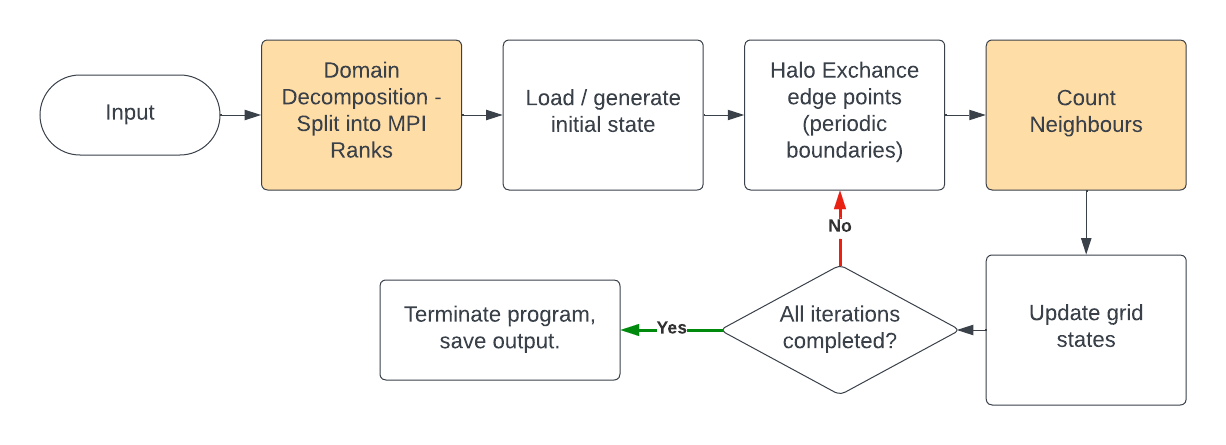
\includegraphics[width=0.9\textwidth]{./figures/high-level-flowchart}
    \caption{A high-level flow chart depicting the algorithm. The key points for efficiency considerations
    are highlighted in red, the considerations are discussed in the main text.}
    \label{fig:high-level-flowchart}
    \end{figure}

    Fig.\eqref{fig:high-level-flowchart} shows the high-level algorithm being used to simulate Conway's
    Game of Life.
    The key points of consideration with regard to performance are highlighted in red.
    There are 3 domain decomposition methods available (column, row and block decomposition) as well as multiple
    ways to count neighbours and update grid states.
    As indicated in Fig.\eqref{fig:high-level-flowchart}, communication overheads between MPI ranks can be hidden
    behind computation by using non-blocking communication and counting whichever neighbours are available at the time.
    Likewise, the actual method of counting neighbours and updating the grid can be done in a variety of ways, each with
    their own merits.
    All these considerations are discussed thoroughly in this section, and then they are investigated in the next
    section.

    \subsection{Domain Decomposition and Neighbour Counting Algorithm}\label{subsec:domain-decomp}
    Domain decomposition can be done by either strips or blocks.
    Strips has the advantage that it is simpler to implement but will have more memory needing to be passed between
    boundaries, with the opposite being true for blocks.
    Therefore, the choice of domain decomposition will need to be tested to see which is more efficient as the data
    size and number of MPI ranks increases.
    However, the overheads of communication can be effectively nullified if the communication is hidden behind computation,
    as such, this also needs to be explored to see what proportion of the communication can be hidden.

    The neighbour counting algorithm has 2 possible implementations, a simple convolution and a separable kernel.
    \begin{itemize}
        \item \textbf{Simple convolution.} Loop through each cell, and count the number of neighbours.
            This is equivalent to a 3x3 convolution with the below kernel.
            \begin{equation}
            \begin{bmatrix}
            1 & 1 & 1 \\
            1 & 0 & 1 \\
            1 & 1 & 1 \\
            \end{bmatrix}\label{eq:kernel1}
            \end{equation}
            This requires a total of $8N^{2}$ addition operations (the $9N^{2}$ multiplication operations that would usually occur can
            be ignored because the kernel only contain 1s and 0s so we can skip the multiplication operation in this special case).
        \item \textbf{Separable kernel.} If the following kernel is used instead,
            \begin{equation}
            \begin{bmatrix}
            1 & 1 & 1 \\
            1 & 1 & 1 \\
            1 & 1 & 1 \\
            \end{bmatrix}\label{eq:kernel2}
            \end{equation}
            then the kernel becomes separable.
            This means that the kernel can be split into two 1D identical kernels \(\begin{bmatrix} 1 & 1 & 1 \end{bmatrix}\) and
            applied in two passes which yields $2N^{2}$ addition operations per pass, yielding a total of $4N^{2}$ operations \cite{separable-kernel}.
            After another ${N^{2}}$ addition operations, to correct for replacing the central 0 with a 1, the total number of
            operations becomes $5N^{2}$.
            Therefore, the separable kernel method yields a theoretical speedup of $8/5 \approx 1.6$.
            However, due to strided memory access on the vertical pass, the speedup will be less than this.
            Although, the vertical pass can be made more efficient by transposing the grid and making the data contiguous,
            it will need to be investigated whether the additional overhead of transposing the grid yields any speedup.
    \end{itemize}

    The simple convolution method would prefer column-wise decomposition as it would reduce the number of cache misses
    when counting the 6 neighbours that are not horizontally adjacent to the current cell.
    This is because shorter rows would reduce the distance in memory between a cell and it's vertical neighbour.
    Theoretically, the separable kernel should not have this issue if the separable convolution can be applied in two horizontal
    passes with a transpose in between.

    \subsection{Hiding Communication Behind Computation}\label{subsec:hiding-comms}
    To the extent of hiding communication behind computation, the separable convolution allows naturally for the horizontal
    pass to be done first, and then the vertical pass to be done after the vertical halos have been exchanged.
    Doing the vertical pass first is also possible but likely to be less efficient due to the strided memory access.
    This would, however, only hide communication if the horizontal halos arrive before the vertical halos which is not guaranteed.
    Given that the horizontal halo exchange involves the exchange of non-contiguous data (assuming the grid is represented
    as a 1D array in row-major order), unless the horizontal halos are smaller than the vertical halos (which would be
    the case in row decomposition), the communication will likely not be hidden behind computation.
    There are other factors such as physical positioning of the MPI ranks and the network topology that will also affect
    the communication overheads between MPI ranks, so it is hard to predict how much time could be consistently saved by
    hiding communication in this method.

    The alternative option for hiding communication is to count the neighbours with the simple convolution
    for all the cells that are not on the boundary, and then count the neighbours for the cells on the boundary once the halo
    exchange has been completed.
    The downside of this is that it involves a lot of non-contiguous memory access, which is not ideal for performance, but
    how this method compares to the previous method as the simulation scaled will need to be investigated.

    \subsection{Updating Grid}\label{subsec:update-grid}
    Given the neighbour count and the current state of the grid, there are a few possible ways to update the grid \cite{branchless-programming}.
    \begin{itemize}
        \item \textbf{\inlinecode{if} statements.} This is the most straightforward implementation.
        The minimum number of \inlinecode{if} statements required to implement the rules of Conway's Game of Life is 3,
        and it is unlikely the CPU will be able to optimise this to any degree with branch prediction, so
        this method will likely be the slowest.
        \item \textbf{Bitwise operations.} This method removes all \inlinecode{if} statements and replaces them with
            inline bitwise (\inlinecode{&&} and \inlinecode{||}) operations.
        \item \textbf{Lookup table.} Given that there is only 18 states a cell can be in (dead or alive, with 0 to 8 neighbours),
            a lookup array can be used to update the grid with the new state of each cell, given one of the current
            18 states.
    \end{itemize}
    The efficacy of these methods will need to be tested to see which is the most efficient.

    \subsection{OpenMP with MPI}\label{subsec:omp-with-mpi}
    The final consideration is to assess how to use OpenMP with MPI.
    Not all loops will be infinitely parallelisable, more threads won't always yield a linear speedup.
    Likewise, more MPI ranks yields more communication overheads, and as such there will be trade-offs in this respect.
    The trade-off between OpenMP and MPI will need to be investigated empirically to see what the best combination is.




%! Author = adnansiddiquei
%! Date = 08/03/2024

\section{Development, Experimentation, Profiling and Optimisation}\label{sec:development}
    This section discusses the experimentation and profiling of the different methods discussed in the previous
    section (Section \eqref{sec:prototyping}).
    Most of the experimentation was done on a Macbook M1 Pro (10 cores; 16GB RAM; 128 KB of L1 data cache; 192 KB of L1
    instruction cache; 64 Byte cache line size; 4 MB of L2 cache), which is why the number of OpenMP threads for local
    experimentation was limited to 10.
    \subsection{Profiling the Convolution Methods}\label{subsec:prof-conv}
    \begin{figure}[htb]
    \centering
    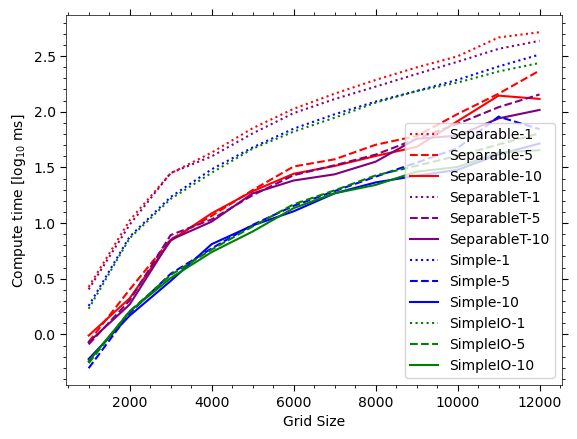
\includegraphics[width=0.75\textwidth]{./figures/convolutions}
    \caption{A figure showing the compute time for 4 of the convolution methods for counting neighbours.
        The colour of the line indicates the method used, and the line style (dotted, dashed, solid) indicates the number
        OpenMP threads used (1, 5 and 10 respectively).
        Only 1 MPI rank was used.
        The x-axis shows the size of one dimension of the square grid.
        The Simple and Separable methods are as described in \eqref{subsec:domain-decomp} and the SimpleIO method is
        as described in \eqref{subsec:hiding-comms})
        The SeparableT method is the Separable method done in 2 horizontal passes with a transpose in between, except
        the time on the graph is just the compute time to repeast the first horizontal pass twice (i.e, it is the time
        for the actual SeparableT method minus the tranpose compute time).
        This was done for simplicity, to assess whether a tranpose operation needed coding.
        The compute time is averaged over 3 runs.}
    \label{fig:convolutions}
    \end{figure}

    Fig.\eqref{fig:convolutions} shows the compute time across 4 different convolution methods for counting neighbours
    and how they scale with \inlinecode{grid_size} and \inlinecode{OMP_NUM_THREADS}.
    The first observation is that both the simple methods are faster than both of the separable methods, which is
    at face value, unexpected.
    Furthermore, there is a negligible difference in speed between the Simple and SimpleIO method which is a positive
    outcome which means the SimpleIO method is a good candidate for hiding communication overheads, as the vast majority
    of the computation can be done while waiting for the communication to complete.
    It is worth noting that all of these methods show diminishing returns as the number of OMP threads increases.
    \begin{figure}[htb]
    \centering
    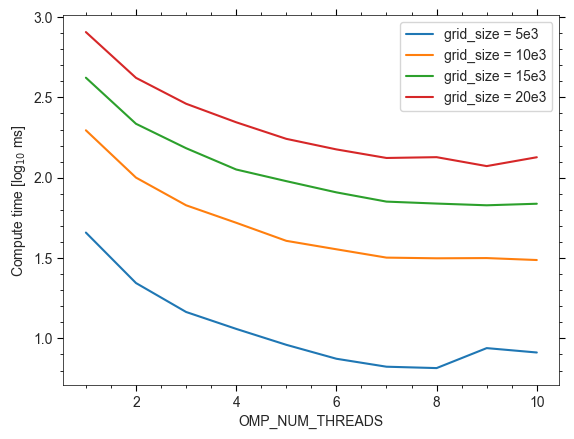
\includegraphics[width=0.75\textwidth]{./figures/simpleio}
    \caption{A figure showing how the compute time varies for the SimpleIO method as the number of OMP threads is changed.
    1 MPI rank was used, and compute time is averaged over 3 runs.}
    \label{fig:simpleio}
    \end{figure}

    Fig.\eqref{fig:simpleio} shows that as the number of OMP threads increases, the compute time decreases, but with
    diminishing returns.
    The jump from 1 to 2 threads yields a 2x increase but jumps following this do not yield speed increases in the same
    proportion.
    At about 8 threads, the returns on increasing the number of threads become negligible, which is useful information
    for optimising the MPI rank to OMP thread ratio.

    The analysis thus far has yielded the following conclusions: the SimpleIO method is a good candidate for counting
    neighbours and hiding MPI communication overheads; and 8 may be a reasonable cap on the optimal number of OMP threads.

    \subsection{Profiling the Update Methods}\label{subsec:prof-trans}
        \begin{figure}[htb]
    \centering
    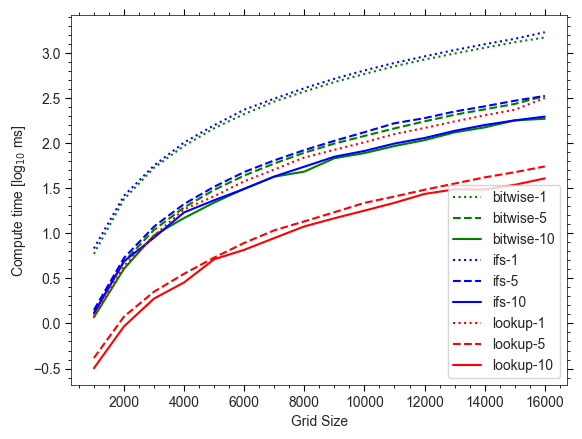
\includegraphics[width=0.75\textwidth]{./figures/transitions}
    \caption{A figure showing the compute time for the 3 the update methods discussed in Section \eqref{subsec:update-grid}.
        The colour of the line indicates the method used, and the line style (dotted, dashed, solid) indicates the number
        OpenMP threads used (1, 5 and 10 respectively).
        Only 1 MPI rank was used.
        The compute time is averaged over 3 runs.}
    \label{fig:transitions}
    \end{figure}

    Fig.\eqref{fig:transitions} explores the update methods discussed in Section \eqref{subsec:update-grid}, with a
    clear conclusion that the lookup method is the fastest, and as expected, the \inlinecode{if} method is the slowest.
    This makes sense, due to the (effectively) random nature of the simulation, the CPU will have little success
    in branch predictions, contributing to the slowness of the \inlinecode{if} method down.
    The frequent lookup in an 18-length array is relatively inexpensive compared to frequent branching.





%! Author = adnansiddiquei
%! Date = 08/03/2024

\section{Experimentation, Profiling and Optimisation}\label{sec:profiling}
    This section discusses the experimentation and profiling of the different methods discussed in Section \eqref{sec:prototyping}.
    Most of the experimentation was done on a Macbook M1 Pro (see Appendix \eqref{app:macbook-specs}), which is why the number of OpenMP threads for local
    experimentation was limited to 10.
    \subsection{Profiling the Convolution Methods}\label{subsec:prof-conv}
    \begin{figure}[htb]
    \centering
    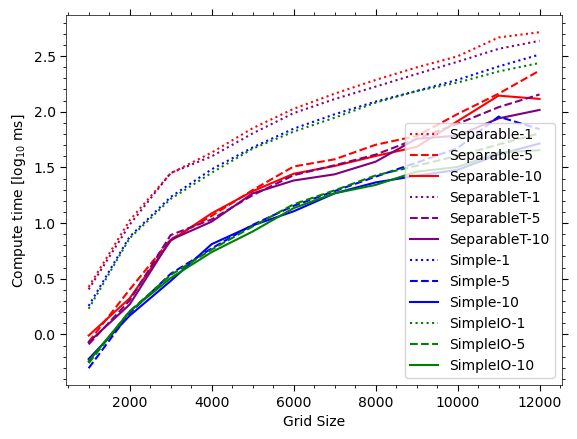
\includegraphics[width=0.75\textwidth]{./figures/convolutions}
    \caption{A figure showing the compute time for 4 of the convolution methods for counting neighbours.
        The colour of the line indicates the method used, and the line style (dotted, dashed, solid) indicates the number
        OpenMP threads used (1, 5 and 10 respectively).
        Only 1 MPI rank was used.
        The x-axis shows the size of one dimension of the square grid.
        The Simple and Separable methods are as described in \eqref{subsec:domain-decomp} and the SimpleIO method is
        as described in \eqref{subsec:hiding-comms})
        The SeparableT method is the Separable method done in 2 horizontal passes with a transpose in between, except
        the time on the graph is just the compute time to repeat the first horizontal pass twice (i.e, it is the time
        for the actual SeparableT method minus the tranpose compute time).
        This was done for simplicity, to assess whether a tranpose operation needed coding.
        The compute time is averaged over 3 runs.}
    \label{fig:convolutions}
    \end{figure}

    Fig.\eqref{fig:convolutions} shows the compute time across 4 different convolution methods for counting neighbours
    and how they scale with \inlinecode{grid_size} and \inlinecode{OMP_NUM_THREADS}.
    The first observation is that both the simple methods are faster than both of the separable methods, which is
    at face value, unexpected.
    Furthermore, there is a negligible difference in speed between the Simple and SimpleIO method which is a positive
    outcome which means the SimpleIO method is a good candidate for hiding communication overheads, as the vast majority
    of the computation can be done while waiting for the communication to complete.
    It is worth noting that all of these methods show diminishing returns as the number of OMP threads increases.

    Loop unrolling was implemented in all of these convolutions, the kernel was applied
    to the grid manually rather than having an additional loop (0 to 8) which applied the kernel.
    Experimentally, this was found to yield about a 2.5x speedup (for the sake of brevity, no figures were generated to
    supplement this conclusion).
    Additionally, all of these double nested loops (which looped over the rows and columns of the grids) were parallelised
    using the OMP \inlinecode{parallel for collapse} clause which allowed OMP to collapse and parallelise the
    nested loops.

    \begin{figure}[htb]
    \centering
    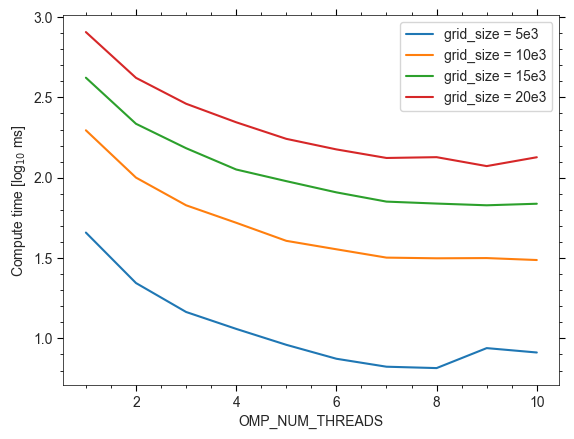
\includegraphics[width=0.75\textwidth]{./figures/simpleio}
    \caption{A figure showing how the compute time varies for the SimpleIO method as the number of OMP threads is changed.
    1 MPI rank was used, and compute time is averaged over 3 runs.}
    \label{fig:simpleio}
    \end{figure}

    Fig.\eqref{fig:simpleio} shows that as the number of OMP threads increases, the compute time decreases, but with
    diminishing returns.
    The jump from 1 to 2 threads yields a 2x increase but jumps following this do not yield speed increases in the same
    proportion.
    At about 8 threads, the returns on increasing the number of threads become negligible, which is useful information
    for optimising the MPI rank to OMP thread ratio.

    The analysis thus far has yielded the following conclusions: the SimpleIO method is a good candidate for counting
    neighbours and hiding MPI communication overheads; and 8 may be a reasonable cap on the optimal number of OMP threads
    (at least, for the M1 Pro chip).

    \subsection{Profiling the Update Methods}\label{subsec:prof-trans}
    \begin{figure}[htb]
    \centering
    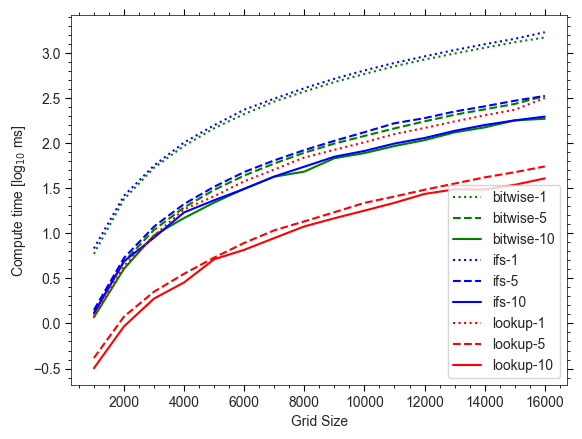
\includegraphics[width=0.75\textwidth]{./figures/transitions}
    \caption{A figure showing the compute time (the time taken to update the entire grid once) for the 3 the update methods
        discussed in Section \eqref{subsec:update-grid}.
        The colour of the line indicates the method used, and the line style (dotted, dashed, solid) indicates the number
        OpenMP threads used (1, 5 and 10 respectively).
        Only 1 MPI rank was used.
        The compute time is averaged over 3 runs.}
    \label{fig:transitions}
    \end{figure}

    Fig.\eqref{fig:transitions} explores the update methods discussed in Section \eqref{subsec:update-grid}, with a
    clear conclusion that the lookup method is the fastest, and as expected, the \inlinecode{if} method is the slowest.
    This makes sense, due to the (effectively) random nature of the simulation, the CPU will have little success
    in branch predictions, contributing to the slowness of the \inlinecode{if} method.
    The frequent lookup in an 18-length array is relatively inexpensive compared to frequent branching.

    \begin{figure}[htb]
    \centering
    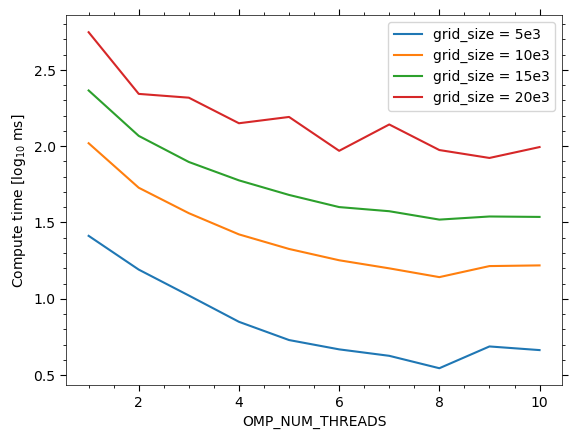
\includegraphics[width=0.75\textwidth]{./figures/lookup}
    \caption{A figure showing how the compute time varies for the updating the grid using the lookup method as the number
        of OMP threads is changed.
        1 MPI rank was used, and compute time is averaged over 5 runs.}
    \label{fig:lookup}
    \end{figure}

    Similar to Fig.\eqref{fig:simpleio}, Fig.\eqref{fig:lookup} shows that the lookup method for updating the grid starts
    to show diminishing returns in performance after about 8 OMP threads have been created.

    \subsection{Algorithm Conclusions}\label{subsec:interim-conclusions}
    \begin{figure}[htb]
    \centering
    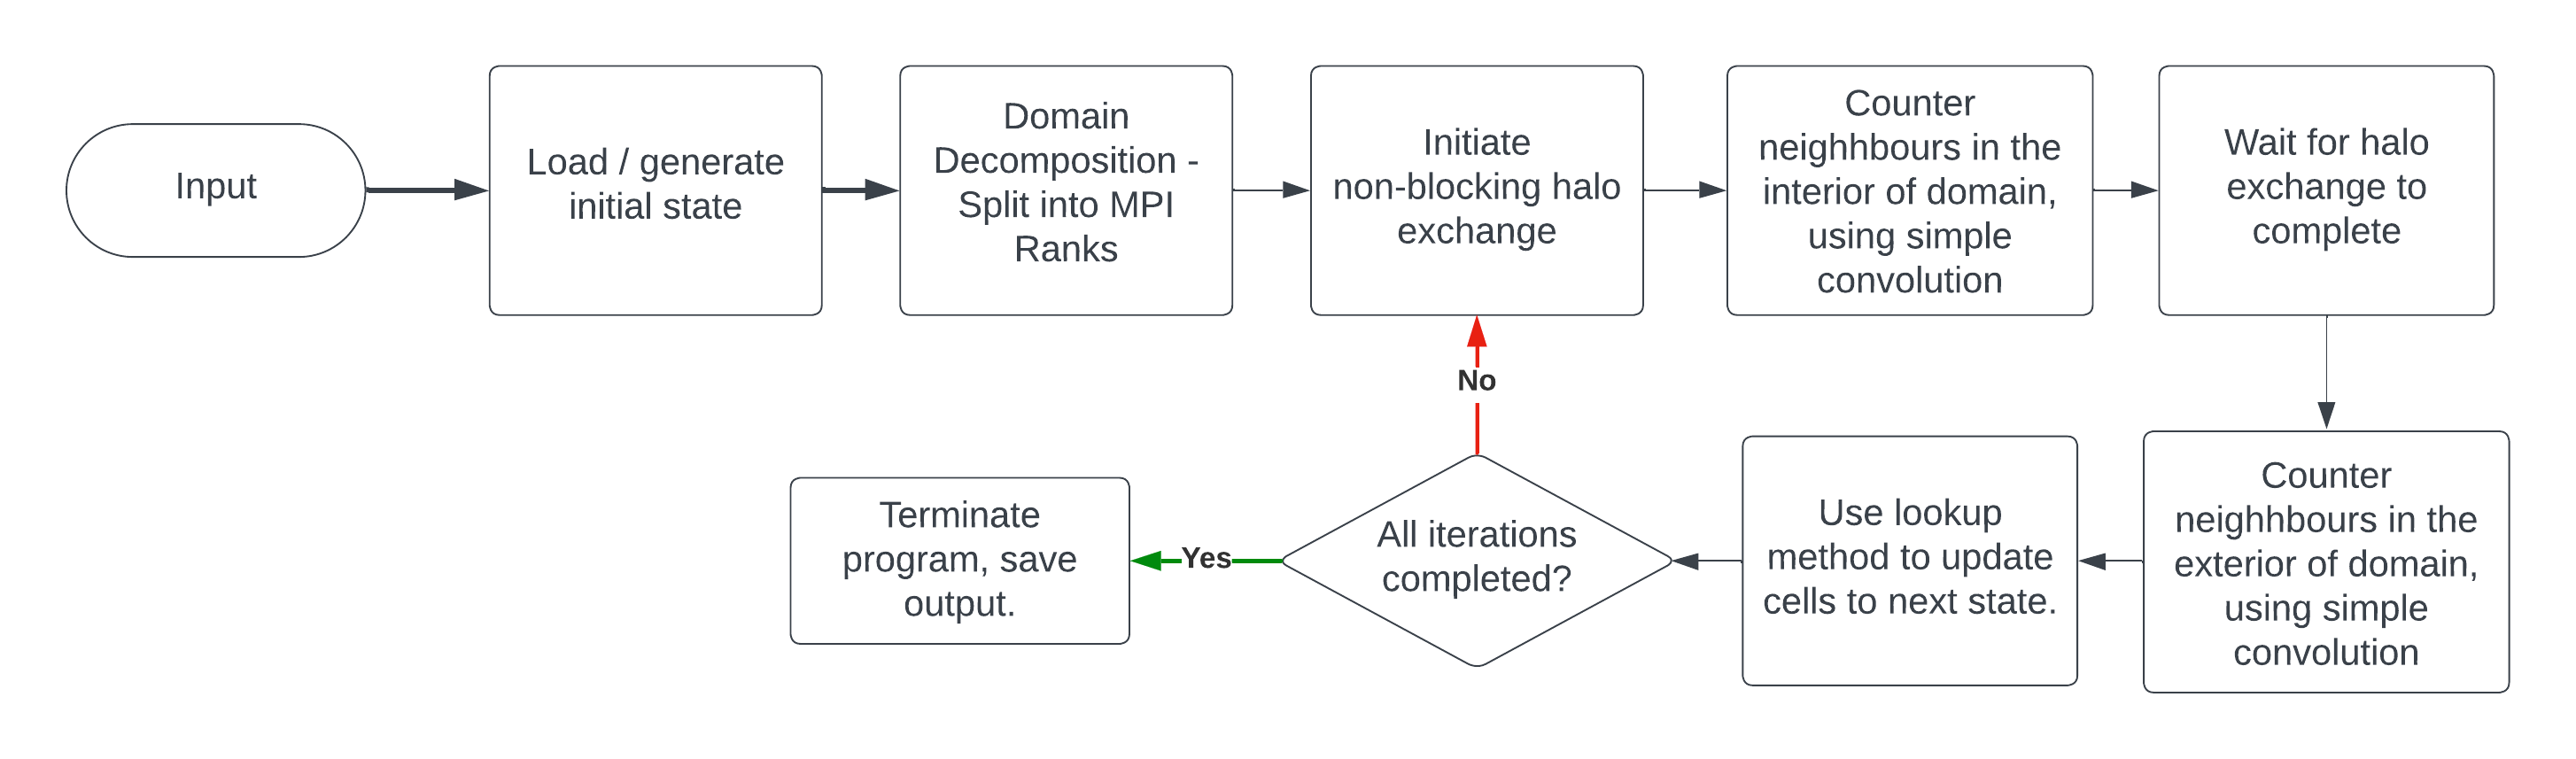
\includegraphics[width=0.9\textwidth]{./figures/flowchat-2}
    \caption{An updated version of Fig.\eqref{fig:high-level-flowchart} with the conclusions from the experimentation
    and profiling.}
    \label{fig:flowhcart-2}
    \end{figure}
    Given the performance testing of the neighbour counting and grid updating methods, the SimpleIO and lookup methods
    are the best candidates for the simulation.
    The SimpleIO can be used to hide communication overheads effectively and the lookup method is the fastest way to
    update the grid, Fig \eqref{fig:flowhcart-2} shows an updated flowchart of the overall algorithm.
    These conclusions are likely transferable to other architectures, but the exact number of OMP threads that yield
    the best performance will need to be re-evaluated for each architecture.
    It is likely that for the M1 Pro, the bottleneck at roughly 8 OMP threads is due to memory constraints rather
    than the algorithm itself not parallelising well, given that the datasets used in the simulation are large enough
    to completely fill L1 and shared L2 caches.

    The optimal domain decomposition was not explored due to time constraints, row-wise decomposition was implemented
    for the sake of simplicity and it was preferred over column-wise decomposition to reduce non-contiguous data transfer
    in the halo exchange.
    The last thing to explore is the optimal number of MPI ranks to use, and the optimal ratio of MPI ranks to OMP threads.

    \subsection{MPI Ranks and OMP Threads}\label{subsec:mpi-omp}
    \begin{figure}[htb]
    \centering
    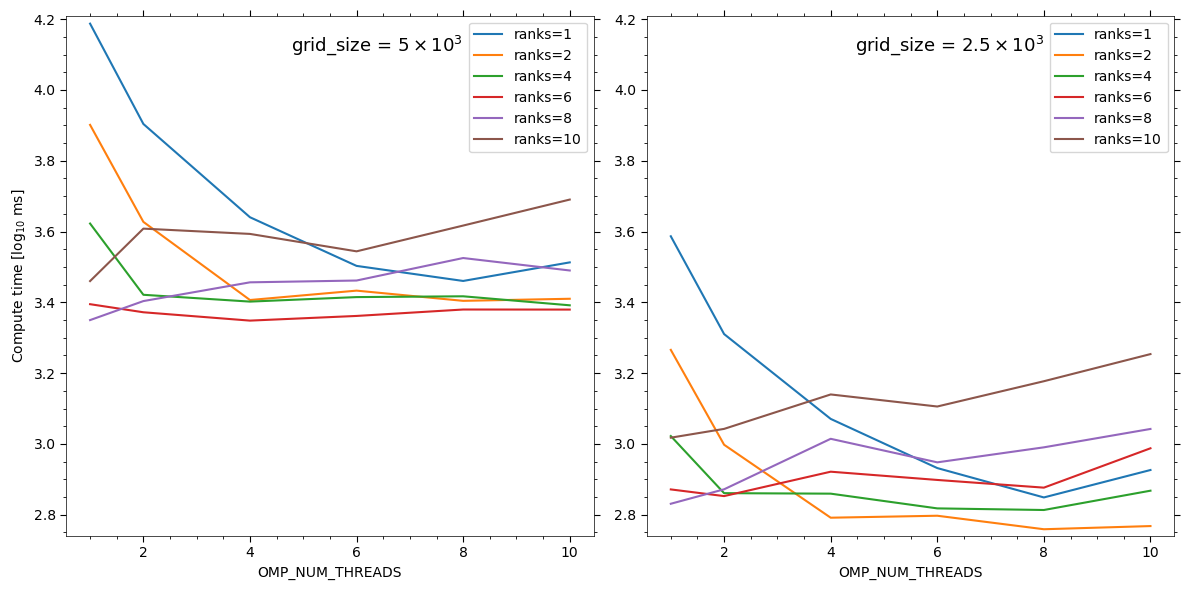
\includegraphics[width=1\textwidth]{./figures/mpi_vs_omp_mac}
    \caption{Two plots illustrating the compute time for the simulation across various number of MPI ranks and OMP threads.
        The left plot is computed with a grid size of 5000, and the right is computed with a grid size of 2500. Both are
        timed over 200 generations and averaged over 2 runs.}
    \label{fig:mpi_vs_omp_mac}
    \end{figure}

    Fig.\eqref{fig:mpi_vs_omp_mac} illustrates the dynamic between the number of MPI ranks and OMP threads on the compute time
    on a Macbook M1 Pro.
    TODO : Run something like this on the HPC. And get some results for that and discuss.








\clearpage
\appendix

\section{Macbook M1 Pro Chip Specifications}\label{app:macbook-specs}
The M1 pro chip has \cite{apple-m1}:
\begin{itemize}
    \item 10 cores; 8 high-performance cores and 2 high-efficiency cores;
    \item Performance cores have 192KB + 128KB L1 instruction + data cache;
    \item Efficiency cores have 128KB + 64KB L1 instruction + data cache;
    \item L1 line size is 64 bytes;
    \item The 8 high-performance cores are divided into 2 clusters, each cluster sharing a 12MB L2 cache;
    \item The 2 high-efficiency cores share a 4MB L2 cache;
    \item 16GB RAM;
\end{itemize}



\begin{thebibliography}{99}

\bibitem{separable-kernel}
Steve Eddins,
\textit{Steve on Image Processing with MATLAB}.
Available at: \url{https://blogs.mathworks.com/steve/2006/10/04/separable-convolution/}
[Accessed: 8-Mar-2024].

\bibitem{branchless-programming}
Srdjan Delić,
\textit{Branchless programming — Why your CPU will thank you}.
Available at: \url{https://sdremthix.medium.com/branchless-programming-why-your-cpu-will-thank-you-5f405d97b0c8}
[Accessed: 17-Mar-2024].

\bibitem{apple-m1}
Wikipedia,
\textit{Apple M1}.
Available at: \url{https://en.wikipedia.org/wiki/Apple_M1}
[Accessed: 17-Mar-2024].



\end{thebibliography}



\end{document}
